\documentclass{standalone}
\usepackage{tikz}
\usetikzlibrary{shapes.misc, arrows.meta, positioning, bending, fit}

\begin{document}
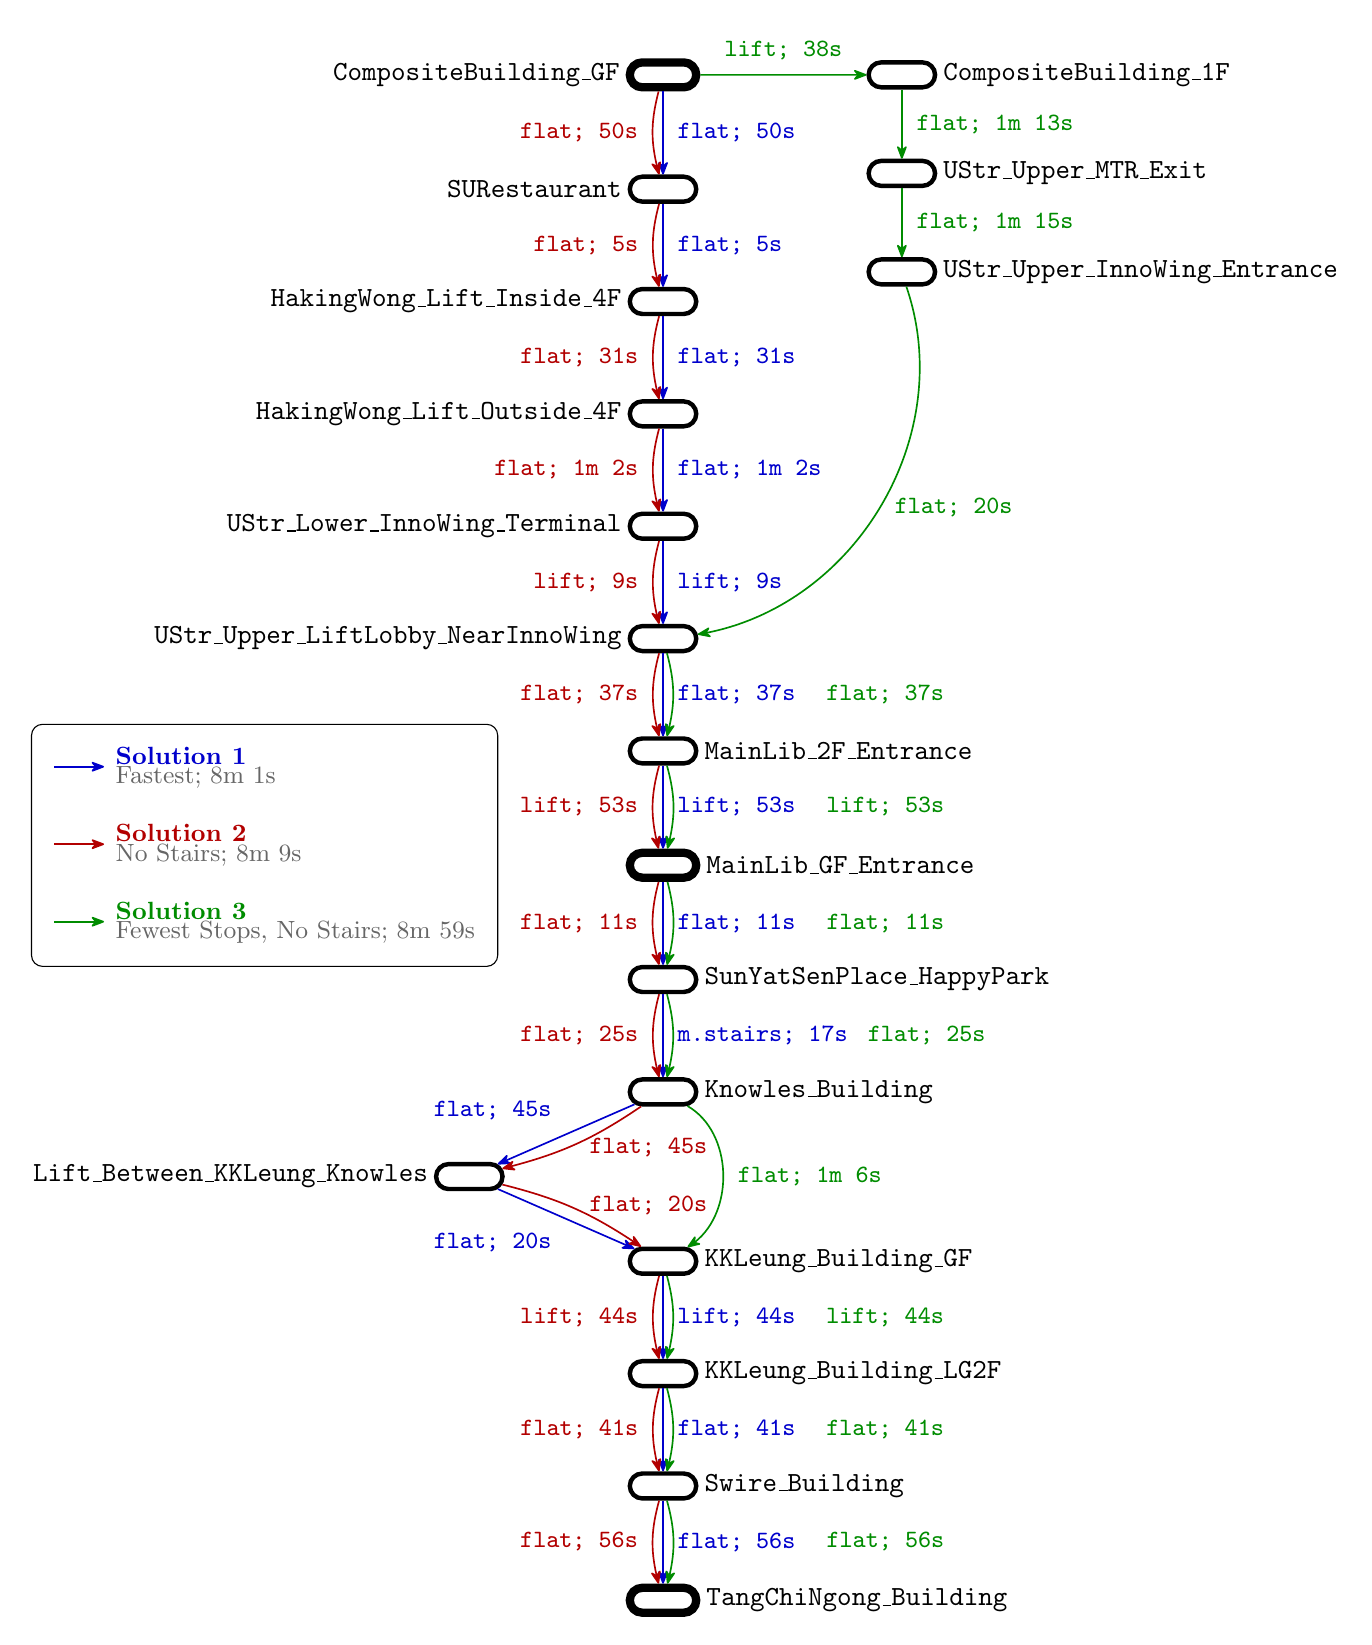
\begin{tikzpicture}[
    %% ── Node styles ──────────────────────────────────────────────────────
    %%
    %% station: small pill/stadium shape used as the "dot" indicator.
    %%   The node body is EMPTY; the monospaced name lives OUTSIDE as a label.
    %%   Edges and positioning are anchored to the pill shape, not the text.
    %%
    %%   Usage:
    %%     \node[station, label={[stlabel]right:NODE\_ID}]               (A) {};
    %%     \node[station-bold, label={[stlabel-bold]right:NODE\_ID}]     (A) {};
    %%
    station/.style={
        draw,
        shape=rounded rectangle,   % from shapes.misc — true semi-circular ends
        rounded rectangle arc length=180,
        minimum height=0.9em,       % height sets the semicircle diameter
        minimum width=2.4em,        % must exceed height to get a flat middle section
        inner xsep=0pt,
        inner ysep=0pt,
        line width=1.6pt,
    },
    %% station-bold + stlabel-bold: use on start/end/waypoint nodes for emphasis.
    station-bold/.style={station, line width=3pt},
    %% stlabel: monospaced name label placed to the right of the station dot.
    %%   Always pass it as the style argument to the label option:
    %%     label={[stlabel]right:NAME}
    stlabel/.style={font=\ttfamily, inner sep=2pt},
    stlabel-bold/.style={stlabel, font=\ttfamily\bfseries},
    %% ── Base directed edge style ───────────────────────────────────────────────
    %%
    %%   All per-solution styles inherit from this.
    %%   For parallel edges use bend left/right:
    %%     \draw[sol1, bend left=20] (A) to node[elabel, above] {label} (B);
    route/.style={
        ->,
        >=Stealth[round],
        semithick,
        % shorten >=4pt,
        % shorten <=4pt,
    },
    %% ── Per-solution edge styles (one colour per solution) ────────────
    %%
    %%   Usage:  \draw[sol1] (A) -- (B);
    %%           \draw[sol2, bend left=20] (A) to node[elabel, above] {text} (B);
    sol1/.style={route, color=blue!80!black},           % Solution 1 — blue
    sol2/.style={route, color=red!70!black},            % Solution 2 — red
    sol3/.style={route, color=green!55!black},          % Solution 3 — green
    sol4/.style={route, color=orange!85!black},         % Solution 4 — orange
    sol5/.style={route, color=violet!80!black},         % Solution 5 — violet
    %% ── Edge label styles ────────────────────────────────────────────────
    %%
    %%   Use the per-solution variant (elabel1–elabel5) so that identical labels
    %%   on parallel edges are still distinguishable by colour.
    %%
    %%   For N parallel edges on the same node pair, spread them symmetrically:
    %%     N=2: bend left=15  /  bend right=15
    %%     N=3: bend left=25  /  straight (no bend)  /  bend right=25
    %%     N=4: bend left=35  /  bend left=12  /  bend right=12  /  bend right=35
    %%
    %%   To additionally separate labels, use xshift on the node option:
    %%     node[elabel3, right, xshift=8pt]
    %%
    %%   Example (2 parallel edges):
    %%     \draw[sol1, bend left=15]  (A) to node[elabel1, left]  {label} (B);
    %%     \draw[sol2, bend right=15] (A) to node[elabel2, right] {label} (B);
    %% ── Legend styles ──────────────────────────────────────────────────────
    %%
    %%   legendtitle: bold coloured solution name — pair with the solution colour.
    %%     e.g. \node[legendtitle, text=blue!80!black] {Solution 1};
    legendtitle/.style={font=\small\bfseries, inner sep=0pt, anchor=west},
    %%   legenddesc: smaller grey text for the lines below the title.
    legenddesc/.style={font=\small, text=black!60, inner sep=0pt, anchor=west},
    elabel/.style ={font=\small\ttfamily, inner sep=5pt},
    elabel1/.style={elabel, text=blue!80!black},
    elabel2/.style={elabel, text=red!70!black},
    elabel3/.style={elabel, text=green!55!black},
    elabel4/.style={elabel, text=orange!85!black},
    elabel5/.style={elabel, text=violet!80!black},
]

%% ── Nodes ────────────────────────────────────────────────────────────────

%% Sol1/Sol2 main spine (left column)
\node[station-bold, label={[stlabel-bold]left:CompositeBuilding\_GF}]
    (CompositeBuilding_GF) {};
\node[station, label={[stlabel]left:SURestaurant},
    below=30pt of CompositeBuilding_GF]
    (SURestaurant) {};
\node[station, label={[stlabel]left:HakingWong\_Lift\_Inside\_4F},
    below=30pt of SURestaurant]
    (HakingWong_Lift_Inside_4F) {};
\node[station, label={[stlabel]left:HakingWong\_Lift\_Outside\_4F},
    below=30pt of HakingWong_Lift_Inside_4F]
    (HakingWong_Lift_Outside_4F) {};
\node[station, label={[stlabel]left:UStr\_Lower\_InnoWing\_Terminal},
    below=30pt of HakingWong_Lift_Outside_4F]
    (UStr_Lower_InnoWing_Terminal) {};
\node[station, label={[stlabel]left:UStr\_Upper\_LiftLobby\_NearInnoWing},
    below=30pt of UStr_Lower_InnoWing_Terminal]
    (UStr_Upper_LiftLobby_NearInnoWing) {};  %% Sol3 merges here

%% Sol3 detour: CompositeBuilding_GF → ... → UStr_Upper_LiftLobby_NearInnoWing (right column)
\node[station, label={[stlabel]right:CompositeBuilding\_1F},
    right=60pt of CompositeBuilding_GF]
    (CompositeBuilding_1F) {};
\node[station, label={[stlabel]right:UStr\_Upper\_MTR\_Exit},
    below=25pt of CompositeBuilding_1F]
    (UStr_Upper_MTR_Exit) {};
\node[station, label={[stlabel]right:UStr\_Upper\_InnoWing\_Entrance},
    below=25pt of UStr_Upper_MTR_Exit]
    (UStr_Upper_InnoWing_Entrance) {};

%% Shared from here (all three solutions)
\node[station, label={[stlabel]right:MainLib\_2F\_Entrance},
    below=30pt of UStr_Upper_LiftLobby_NearInnoWing]
    (MainLib_2F_Entrance) {};
\node[station-bold, label={[stlabel-bold]right:MainLib\_GF\_Entrance},
    below=30pt of MainLib_2F_Entrance]
    (MainLib_GF_Entrance) {};   %% Intermediate waypoint
\node[station, label={[stlabel]right:SunYatSenPlace\_HappyPark},
    below=30pt of MainLib_GF_Entrance]
    (SunYatSenPlace_HappyPark) {};
\node[station, label={[stlabel]right:Knowles\_Building},
    below=30pt of SunYatSenPlace_HappyPark]
    (Knowles_Building) {};

%% Sol1/Sol2 go via Lift_Between_KKLeung_Knowles (to the right of Knowles_Building)
%% Sol3 goes directly to KKLeung_Building_GF
\node[station, label={[stlabel]left:Lift\_Between\_KKLeung\_Knowles},
    below left=20pt and 55pt of Knowles_Building]
    (Lift_Between_KKLeung_Knowles) {};
\node[station, label={[stlabel]right:KKLeung\_Building\_GF},
    below right=20pt and 55pt of Lift_Between_KKLeung_Knowles]
    (KKLeung_Building_GF) {};

%% Shared tail (all three solutions)
\node[station, label={[stlabel]right:KKLeung\_Building\_LG2F},
    below=30pt of KKLeung_Building_GF]
    (KKLeung_Building_LG2F) {};
\node[station, label={[stlabel]right:Swire\_Building},
    below=30pt of KKLeung_Building_LG2F]
    (Swire_Building) {};
\node[station-bold, label={[stlabel-bold]right:TangChiNgong\_Building},
    below=30pt of Swire_Building]
    (TangChiNgong_Building) {};

%% ── Sol3 detour edges ────────────────────────────────────────────────────

\draw[sol3](CompositeBuilding_GF)          -- node[elabel3, above]  {lift; 38s}   (CompositeBuilding_1F);
\draw[sol3](CompositeBuilding_1F)          -- node[elabel3, right]  {flat; 1m 13s}(UStr_Upper_MTR_Exit);
\draw[sol3](UStr_Upper_MTR_Exit)           -- node[elabel3, right]  {flat; 1m 15s}(UStr_Upper_InnoWing_Entrance);
\draw[sol3, bend left=50](UStr_Upper_InnoWing_Entrance)  to node[elabel3, right]  {flat; 20s}   (UStr_Upper_LiftLobby_NearInnoWing);

%% ── Sol1/Sol2 main spine edges ───────────────────────────────────────────

\draw[sol1]               (CompositeBuilding_GF)         -- node[elabel1, right]            {flat; 50s}   (SURestaurant);
\draw[sol2, bend right=15](CompositeBuilding_GF)         to node[elabel2, left]             {flat; 50s}   (SURestaurant);

\draw[sol1]               (SURestaurant)                 -- node[elabel1, right]            {flat; 5s}    (HakingWong_Lift_Inside_4F);
\draw[sol2, bend right=15](SURestaurant)                 to node[elabel2, left]             {flat; 5s}    (HakingWong_Lift_Inside_4F);

\draw[sol1]               (HakingWong_Lift_Inside_4F)    -- node[elabel1, right]            {flat; 31s}   (HakingWong_Lift_Outside_4F);
\draw[sol2, bend right=15](HakingWong_Lift_Inside_4F)    to node[elabel2, left]             {flat; 31s}   (HakingWong_Lift_Outside_4F);

\draw[sol1]               (HakingWong_Lift_Outside_4F)   -- node[elabel1, right]            {flat; 1m 2s} (UStr_Lower_InnoWing_Terminal);
\draw[sol2, bend right=15](HakingWong_Lift_Outside_4F)   to node[elabel2, left]             {flat; 1m 2s} (UStr_Lower_InnoWing_Terminal);

\draw[sol1]               (UStr_Lower_InnoWing_Terminal) -- node[elabel1, right]            {lift; 9s}    (UStr_Upper_LiftLobby_NearInnoWing);
\draw[sol2, bend right=15](UStr_Lower_InnoWing_Terminal) to node[elabel2, left]             {lift; 9s}    (UStr_Upper_LiftLobby_NearInnoWing);

%% ── Shared spine after merge (sol1/sol2/sol3) ───────────────────────────
%%    Sol1 straight, sol2 bend right, sol3 bend left

\draw[sol1]               (UStr_Upper_LiftLobby_NearInnoWing) -- node[elabel1, right]             {flat; 37s} (MainLib_2F_Entrance);
\draw[sol2, bend right=15](UStr_Upper_LiftLobby_NearInnoWing) to node[elabel2, left]              {flat; 37s} (MainLib_2F_Entrance);
\draw[sol3, bend left=15] (UStr_Upper_LiftLobby_NearInnoWing) to node[elabel3, right, xshift=50pt]{flat; 37s} (MainLib_2F_Entrance);

\draw[sol1]               (MainLib_2F_Entrance) -- node[elabel1, right]             {lift; 53s} (MainLib_GF_Entrance);
\draw[sol2, bend right=15](MainLib_2F_Entrance) to node[elabel2, left]              {lift; 53s} (MainLib_GF_Entrance);
\draw[sol3, bend left=15] (MainLib_2F_Entrance) to node[elabel3, right, xshift=50pt]{lift; 53s} (MainLib_GF_Entrance);

\draw[sol1]               (MainLib_GF_Entrance) -- node[elabel1, right]             {flat; 11s} (SunYatSenPlace_HappyPark);
\draw[sol2, bend right=15](MainLib_GF_Entrance) to node[elabel2, left]              {flat; 11s} (SunYatSenPlace_HappyPark);
\draw[sol3, bend left=15] (MainLib_GF_Entrance) to node[elabel3, right, xshift=50pt]{flat; 11s} (SunYatSenPlace_HappyPark);

%% SunYatSenPlace_HappyPark → Knowles_Building: sol1=minor stairs, sol2/sol3=flat
\draw[sol1]               (SunYatSenPlace_HappyPark) -- node[elabel1, right]  {m.stairs; 17s} (Knowles_Building);
\draw[sol2, bend right=15](SunYatSenPlace_HappyPark) to node[elabel2, left]   {flat; 25s}     (Knowles_Building);
\draw[sol3, bend left=15] (SunYatSenPlace_HappyPark) to node[elabel3, right, xshift=65pt]{flat; 25s} (Knowles_Building);

%% Sol1/Sol2: Knowles_Building → Lift_Between_KKLeung_Knowles → KKLeung_Building_GF
\draw[sol1](Knowles_Building)              -- node[elabel1, above left] {flat; 45s} (Lift_Between_KKLeung_Knowles);
\draw[sol2](Knowles_Building)              to[bend left=10] node[elabel2, right, yshift=-1pt] {flat; 45s} (Lift_Between_KKLeung_Knowles);
\draw[sol1](Lift_Between_KKLeung_Knowles)  -- node[elabel1, below left] {flat; 20s} (KKLeung_Building_GF);
\draw[sol2](Lift_Between_KKLeung_Knowles)  to[bend left=10] node[elabel2, right, yshift=1pt] {flat; 20s} (KKLeung_Building_GF);

%% Sol3: Knowles_Building → KKLeung_Building_GF directly (bypasses Lift_Between)
\draw[sol3, bend left=60](Knowles_Building) to node[elabel3, right] {flat; 1m 6s} (KKLeung_Building_GF);

%% ── Shared tail (all three solutions) ───────────────────────────────────

\draw[sol1]               (KKLeung_Building_GF)   -- node[elabel1, right]             {lift; 44s} (KKLeung_Building_LG2F);
\draw[sol2, bend right=15](KKLeung_Building_GF)   to node[elabel2, left]              {lift; 44s} (KKLeung_Building_LG2F);
\draw[sol3, bend left=15] (KKLeung_Building_GF)   to node[elabel3, right, xshift=50pt]{lift; 44s} (KKLeung_Building_LG2F);

\draw[sol1]               (KKLeung_Building_LG2F) -- node[elabel1, right]             {flat; 41s} (Swire_Building);
\draw[sol2, bend right=15](KKLeung_Building_LG2F) to node[elabel2, left]              {flat; 41s} (Swire_Building);
\draw[sol3, bend left=15] (KKLeung_Building_LG2F) to node[elabel3, right, xshift=50pt]{flat; 41s} (Swire_Building);

\draw[sol1]               (Swire_Building) -- node[elabel1, right]             {flat; 56s} (TangChiNgong_Building);
\draw[sol2, bend right=15](Swire_Building) to node[elabel2, left]              {flat; 56s} (TangChiNgong_Building);
\draw[sol3, bend left=15] (Swire_Building) to node[elabel3, right, xshift=50pt]{flat; 56s} (TangChiNgong_Building);

%% ── Legend ───────────────────────────────────────────────────────────────

\begin{scope}[shift={(-220pt, -250pt)}]
    \node[inner sep=0, minimum size=0] (leg-orig) at (0, 0) {};
    \draw[sol1] (0, 0) -- (1.8em, 0);
    \node[legendtitle, text=blue!80!black] (li1-title) at (2.2em,  0.4em) {Solution 1};
    \node[legenddesc]                      (li1-desc)  at (2.2em, -0.4em) {Fastest; 8m 1s};

    \draw[sol2] (0, -2.8em) -- (1.8em, -2.8em);
    \node[legendtitle, text=red!70!black]  (li2-title) at (2.2em, -2.8em+0.4em) {Solution 2};
    \node[legenddesc]                      (li2-desc)  at (2.2em, -2.8em-0.4em) {No Stairs; 8m 9s};

    \draw[sol3] (0, -5.6em) -- (1.8em, -5.6em);
    \node[legendtitle, text=green!55!black](li3-title) at (2.2em, -5.6em+0.4em) {Solution 3};
    \node[legenddesc]                      (li3-desc)  at (2.2em, -5.6em-0.4em) {Fewest Stops, No Stairs; 8m 59s};

    \node[draw, rounded corners=4pt, inner sep=8pt,
          fit=(leg-orig)(li1-title)(li1-desc)(li2-title)(li2-desc)(li3-title)(li3-desc)
    ] {};
\end{scope}

\end{tikzpicture}
\end{document}
